% Judul dokumen
\title{Buku Tugas Akhir ITS}
\author{Musk, Elon Reeve}

% Pengaturan ukuran teks dan bentuk halaman dua sisi
\documentclass[12pt,twoside]{report}

% Pengaturan ukuran halaman dan margin
\usepackage[a4paper,top=30mm,left=30mm,right=20mm,bottom=25mm]{geometry}

% Pengaturan ukuran spasi
\usepackage[singlespacing]{setspace}

% Pengaturan detail pada file PDF
\usepackage[pdfauthor={\@author},bookmarksnumbered,pdfborder={0 0 0}]{hyperref}

% Pengaturan jenis karakter
\usepackage[utf8]{inputenc}

% Pengaturan pewarnaan
\usepackage[table,xcdraw]{xcolor}

% Pengaturan kutipan artikel
\usepackage[style=apa, backend=biber]{biblatex}

% Package lainnya
\usepackage{changepage}
\usepackage{enumitem}
\usepackage{eso-pic}
\usepackage{txfonts} % Font times
\usepackage{etoolbox}
\usepackage{graphicx}
\usepackage{lipsum}
\usepackage{longtable}
\usepackage{tabularx}
\usepackage{wrapfig}
\usepackage{float}
\usepackage{multirow}

% Definisi untuk "Hati ini sengaja dikosongkan"
\patchcmd{\cleardoublepage}{\hbox{}}{
  \thispagestyle{empty}
  \vspace*{\fill}
  \begin{center}\textit{[Halaman ini sengaja dikosongkan]}\end{center}
  \vfill}{}{}

% Pengaturan penomoran halaman
\usepackage{fancyhdr}
\fancyhf{}
\renewcommand{\headrulewidth}{0pt}
\pagestyle{fancy}
\fancyfoot[LE,RO]{\thepage}
\patchcmd{\chapter}{plain}{fancy}{}{}
\patchcmd{\chapter}{empty}{plain}{}{}

% Command untuk bulan
\newcommand{\MONTH}{%
  \ifcase\the\month
  \or Januari% 1
  \or Februari% 2
  \or Maret% 3
  \or April% 4
  \or Mei% 5
  \or Juni% 6
  \or Juli% 7
  \or Agustus% 8
  \or September% 9
  \or Oktober% 10
  \or November% 11
  \or Desember% 12
  \fi}
\newcommand{\ENGMONTH}{%
  \ifcase\the\month
  \or January% 1
  \or February% 2
  \or March% 3
  \or April% 4
  \or May% 5
  \or June% 6
  \or July% 7
  \or August% 8
  \or September% 9
  \or October% 10
  \or November% 11
  \or December% 12
  \fi}

% Pengaturan format judul bab
\usepackage{titlesec}
\titleformat{\chapter}[display]{\bfseries\Large}{BAB \centering\Roman{chapter}}{0ex}{\vspace{0ex}\centering}
\titleformat{\section}{\bfseries\large}{\MakeUppercase{\thesection}}{1ex}{\vspace{1ex}}
\titleformat{\subsection}{\bfseries\large}{\MakeUppercase{\thesubsection}}{1ex}{}
\titleformat{\subsubsection}{\bfseries\large}{\MakeUppercase{\thesubsubsection}}{1ex}{}
\titlespacing{\chapter}{0ex}{0ex}{4ex}
\titlespacing{\section}{0ex}{1ex}{0ex}
\titlespacing{\subsection}{0ex}{0.5ex}{0ex}
\titlespacing{\subsubsection}{0ex}{0.5ex}{0ex}

% Atur variabel berikut sesuai namanya

% nama
\newcommand{\name}{Alfan Miftah Arzaqi}
\newcommand{\authorname}{Musk, Elon Reeve}
\newcommand{\nickname}{Alfan}
\newcommand{\advisor}{Ahmad Zaini, S.T., M.Sc.}
\newcommand{\coadvisor}{Dr. Eko Mulyanto Yuniarno,S.T.,M.T.}
\newcommand{\examinerone}{-}
\newcommand{\examinertwo}{-}
\newcommand{\examinerthree}{-}
\newcommand{\headofdepartment}{Dr. Supeno Mardi Susiki Nugroho, ST., M.T.}

% identitas
\newcommand{\nrp}{0721 19 4000 0003}
\newcommand{\advisornip}{19750419200212 1 003}
\newcommand{\coadvisornip}{19680601199512 1 009}
\newcommand{\examineronenip}{-}
\newcommand{\examinertwonip}{-}
\newcommand{\examinerthreenip}{-}
\newcommand{\headofdepartmentnip}{19700313199512 1 001}

% judul
\newcommand{\tatitle}{KENDALI \textit{MOBILE ROBOT} BERBASIS POSE TANGAN MENGGUNAKAN \textit{CONVOLUTIONAL NEURAL NETWORK} (CNN)}
\newcommand{\engtatitle}{\emph{MOBILE ROBOT CONTROL BASED ON HAND POSE USING CONVOLUTIONAL NEURAL NETWORK (CNN)}}

% tempat
\newcommand{\place}{Surabaya}

% jurusan
\newcommand{\studyprogram}{Teknik Komputer}
\newcommand{\engstudyprogram}{Computer Engineering}

% fakultas
\newcommand{\faculty}{Teknologi Elektro dan Informatika Cerdas}
\newcommand{\engfaculty}{Intelligent Electrical and Informatics Technology}

% singkatan fakultas
\newcommand{\facultyshort}{FTEIC}
\newcommand{\engfacultyshort}{ELECTICS}

% departemen
\newcommand{\department}{Teknik Komputer}
\newcommand{\engdepartment}{Computer Engineering}

% kode mata kuliah
\newcommand{\coursecode}{EC224801}


\hyphenation{
  ro-ket
  me-ngem-bang-kan
  per-hi-tu-ngan
  tek-no-lo-gi
  di-be-ri-kan
}

% Menambahkan resource daftar pustaka
\addbibresource{pustaka/pustaka.bib}

% Pengaturan format potongan kode
\usepackage{listings}
\definecolor{comment}{RGB}{0,128,0}
\definecolor{string}{RGB}{255,0,0}
\definecolor{keyword}{RGB}{0,0,255}
\lstdefinestyle{codestyle}{
  commentstyle=\color{comment},
  stringstyle=\color{string},
  keywordstyle=\color{keyword},
  basicstyle=\footnotesize\ttfamily,
  numbers=left,
  numberstyle=\tiny,
  numbersep=5pt,
  frame=lines,
  breaklines=true,
  prebreak=\raisebox{0ex}[0ex][0ex]{\ensuremath{\hookleftarrow}},
  showstringspaces=false,
  upquote=true,
  tabsize=2,
}
\lstset{style=codestyle}

% Isi keseluruhan dokumen
\begin{document}

% Sampul luar Bahasa Indonesia
\newcommand\covercontents{sampul/konten-id.tex}
\AddToShipoutPictureBG*{
  \AtPageLowerLeft{
    % Ubah nilai berikut jika posisi horizontal background tidak sesuai
    \hspace{-3.25mm}

    % Ubah nilai berikut jika posisi vertikal background tidak sesuai
    \raisebox{0mm}{
      
\includegraphics[width=\paperwidth,height=\paperheight]{sampul/gambar/sampul-luar.png}
    }
  }
}

% Menyembunyikan nomor halaman
\thispagestyle{empty}

% Pengaturan margin untuk menyesuaikan konten sampul
\newgeometry{
  top=55mm,
  left=30mm,
  right=20mm,
  bottom=20mm
}

\begin{flushleft}

  % Pemilihan font sans serif
  \sffamily

  % Pemilihan warna font putih
  \color{white}

  % Pemilihan font bold
  \fontseries{bx}
  \selectfont
  \begin{spacing}{1.5}
    \input{\covercontents}
  \end{spacing}

\end{flushleft}

\restoregeometry


% Atur ulang penomoran halaman
\setcounter{page}{1}

% Sampul dalam Bahasa Indonesia
\renewcommand\covercontents{sampul/konten-id.tex}
\AddToShipoutPictureBG*{
  \AtPageLowerLeft{
    % Ubah nilai berikut jika posisi horizontal background tidak sesuai
    \hspace{-4mm}

    % Ubah nilai berikut jika posisi vertikal background tidak sesuai
    \raisebox{0mm}{
      
\includegraphics[width=\paperwidth,height=\paperheight]{sampul/gambar/sampul-luar-tipis.png}
    }
  }
}

% Menyembunyikan nomor halaman
\thispagestyle{empty}

% Pengaturan margin untuk menyesuaikan konten sampul
\newgeometry{
  top=65mm,
  left=30mm,
  right=30mm,
  bottom=20mm
}

\begin{flushleft}

  % Pemilihan font sans serif
  \sffamily

  % Pemilihan font bold
  \fontseries{bx}
  \selectfont
  \begin{spacing}{1.5}
    \input{\covercontents}
  \end{spacing}

\end{flushleft}

\restoregeometry

\clearpage
\cleardoublepage

% Sampul dalam Bahasa Inggris
\renewcommand\covercontents{sampul/konten-en.tex}
\AddToShipoutPictureBG*{
  \AtPageLowerLeft{
    % Ubah nilai berikut jika posisi horizontal background tidak sesuai
    \hspace{-4mm}

    % Ubah nilai berikut jika posisi vertikal background tidak sesuai
    \raisebox{0mm}{
      
\includegraphics[width=\paperwidth,height=\paperheight]{sampul/gambar/sampul-luar-tipis.png}
    }
  }
}

% Menyembunyikan nomor halaman
\thispagestyle{empty}

% Pengaturan margin untuk menyesuaikan konten sampul
\newgeometry{
  top=65mm,
  left=30mm,
  right=30mm,
  bottom=20mm
}

\begin{flushleft}

  % Pemilihan font sans serif
  \sffamily

  % Pemilihan font bold
  \fontseries{bx}
  \selectfont
  \begin{spacing}{1.5}
    \input{\covercontents}
  \end{spacing}

\end{flushleft}

\restoregeometry

\cleardoublepage

% Label tabel dan gambar dalam bahasa indonesia
\renewcommand{\figurename}{Gambar}
\renewcommand{\tablename}{Tabel}

% Pengaturan ukuran indentasi paragraf
\setlength{\parindent}{2em}

% Pengaturan ukuran spasi paragraf
\setlength{\parskip}{1ex}

% Lembar pengesahan
\begin{center}
  \large
  \textbf{LEMBAR PENGESAHAN}
\end{center}

% Menyembunyikan nomor halaman
\thispagestyle{empty}

\begin{center}
  \textbf{\tatitle{}}
\end{center}

\begingroup
% Pemilihan font ukuran small
\small

\begin{center}
  \textbf{TUGAS AKHIR}
  \\Diajukan untuk memenuhi salah satu syarat \\
  memperoleh gelar Sarjana Teknik pada \\
  Program Studi S-1 \studyprogram{} \\
  Departemen \department{} \\
  Fakultas \faculty{} \\
  Institut Teknologi Sepuluh Nopember
\end{center}

\begin{center}
  Oleh: \textbf{\name{}}
  \\NRP. \nrp{}
\end{center}

\begin{center}
  Disetujui oleh Tim Penguji Tugas Akhir:
\end{center}

\begingroup
% Menghilangkan padding
\setlength{\tabcolsep}{0pt}

\noindent
\begin{tabularx}{\textwidth}{X l}
  \advisor{}               & (Pembimbing I)                      \\
  NIP: \advisornip{}       &                                     \\
                           & ................................... \\
                           &                                     \\
                           &                                     \\
  \coadvisor{}             & (Pembimbing II)                     \\
  NIP: \coadvisornip{}     &                                     \\
                           & ................................... \\
                           &                                     \\
                           &                                     \\
  \examinerone{}.          & (Penguji I)                         \\
  NIP: \examineronenip{}   &                                     \\
                           & ................................... \\
                           &                                     \\
                           &                                     \\
  \examinertwo{}.          & (Penguji II)                        \\
  NIP: \examinertwonip{}   &                                     \\
                           & ................................... \\
                           &                                     \\
                           &                                     \\
  \examinerthree{}.        & (Penguji III)                       \\
  NIP: \examinerthreenip{} &                                     \\
                           & ................................... \\
\end{tabularx}
\endgroup

\begin{center}
  Mengetahui, \\
  Kepala Departemen \department{} \facultyshort{} - ITS\\

  \vspace{8ex}

  \underline{\headofdepartment{}.} \\
  NIP. \headofdepartmentnip{}
\end{center}

\begin{center}
  \textbf{\MakeUppercase{\place{}}\\\MONTH{}, \the\year{}}
\end{center}
\endgroup

\cleardoublepage
\begin{center}
  \large
  \textbf{APPROVAL SHEET}
\end{center}

% Menyembunyikan nomor halaman
\thispagestyle{empty}

\begin{center}
  \textbf{\engtatitle{}}
\end{center}

\begingroup
% Pemilihan font ukuran small
\small

\begin{center}
  \textbf{FINAL PROJECT}
  \\Submitted to fulfill one of the requirements \\
  for obtaining a degree Bachelor of Engineering at \\
  Undergraduate Study Program of \engstudyprogram{} \\
  Department of \engdepartment{} \\
  Faculty of \engfaculty{} \\
  Sepuluh Nopember Institute of Technology
\end{center}

\begin{center}
  By: \textbf{\name{}}
  \\NRP. \nrp{}
\end{center}

\begin{center}
  Approved by Final Project Examiner Team:
\end{center}

\begingroup
% Menghilangkan padding
\setlength{\tabcolsep}{0pt}

\noindent
\begin{tabularx}{\textwidth}{X l}
  \advisor{}               & (Advisor I)                         \\
  NIP: \advisornip{}       &                                     \\
                           & ................................... \\
                           &                                     \\
                           &                                     \\
  \coadvisor{}             & (Co-Advisor II)                     \\
  NIP: \coadvisornip{}     &                                     \\
                           & ................................... \\
                           &                                     \\
                           &                                     \\
  \examinerone{}.          & (Examiner I)                        \\
  NIP: \examineronenip{}   &                                     \\
                           & ................................... \\
                           &                                     \\
                           &                                     \\
  \examinertwo{}.          & (Examiner II)                       \\
  NIP: \examinertwonip{}   &                                     \\
                           & ................................... \\
                           &                                     \\
                           &                                     \\
  \examinerthree{}.        & (Examiner III)                      \\
  NIP: \examinerthreenip{} &                                     \\
                           & ................................... \\
\end{tabularx}
\endgroup


\begin{center}
  Acknowledged, \\
  Head of \engdepartment{} Department \engfacultyshort{} - ITS \\

  \vspace{8ex}

  \underline{\headofdepartment{}.} \\
  NIP. \headofdepartmentnip{}
\end{center}

\begin{center}
  \textbf{\MakeUppercase{\place{}}\\\ENGMONTH{}, \the\year{}}
\end{center}
\endgroup

\cleardoublepage

% Pernyataan keaslian
\begin{center}
  \large
  \textbf{PERNYATAAN ORISINALITAS}
\end{center}

% Menyembunyikan nomor halaman
\thispagestyle{empty}

\vspace{2ex}

% Ubah paragraf-paragraf berikut sesuai dengan yang ingin diisi pada pernyataan keaslian

\noindent Yang bertanda tangan dibawah ini:

\noindent\begin{tabularx}{\textwidth}{l l X}
                         &   &                            \\
  Nama Mahasiswa / NRP   & : & \name{} / \nrp{}           \\
  Departemen             & : & \department{}              \\
  Dosen Pembimbing / NIP & : & \advisor{} / \advisornip{} \\
                         &   &                            \\
\end{tabularx}

Dengan ini menyatakan bahwa Tugas Akhir dengan judul "\tatitle{}" adalah hasil karya sendiri, berfsifat orisinal, dan ditulis dengan mengikuti kaidah penulisan ilmiah.

Bilamana di kemudian hari ditemukan ketidaksesuaian dengan pernyataan ini, maka saya bersedia menerima sanksi sesuai dengan ketentuan yang berlaku di Institut Teknologi Sepuluh Nopember.

\vspace{8ex}

\noindent\begin{tabularx}{\textwidth}{X l}
                     & \place{}, \ENGMONTH{} \the\year{} \\
                     &                                   \\
  Mengetahui         &                                   \\
  Dosen Pembimbing   & Mahasiswa                         \\
                     &                                   \\
                     &                                   \\
                     &                                   \\
                     &                                   \\
                     &                                   \\
  \advisor{}         & \name{}                           \\
  NIP. \advisornip{} & NRP. \nrp{}                       \\
\end{tabularx}

\cleardoublepage
\begin{center}
  \large
  \textbf{STATEMENT OF ORIGINALITY}
\end{center}

% Menyembunyikan nomor halaman
\thispagestyle{empty}

\vspace{2ex}

% Ubah paragraf-paragraf berikut sesuai dengan yang ingin diisi pada pernyataan keaslian

\noindent The undersigned below:

\noindent\begin{tabularx}{\textwidth}{l l X}
                        &   &                            \\
  Name of student / NRP & : & \name{} / \nrp{}           \\
  Department            & : & \engdepartment{}           \\
  Advisor / NIP         & : & \advisor{} / \advisornip{} \\
                        &   &                            \\
\end{tabularx}

Hereby declared that the Final Project with the title of "\engtatitle{}" is the result of my own work, is original, and is written by following the rules of scientific writing.

If in future there is a discrepancy with this statement, then I am willing to accept sanctions in accordance with provisions that apply at Sepuluh Nopember Institute of Technology.

\vspace{8ex}

\noindent\begin{tabularx}{\textwidth}{X l}
                     & \place{}, \ENGMONTH{} \the\year{} \\
                     &                                   \\
  Acknowledged       &                                   \\
  Advisor            & Student                           \\
                     &                                   \\
                     &                                   \\
                     &                                   \\
                     &                                   \\
                     &                                   \\
  \advisor{}         & \name{}                           \\
  NIP. \advisornip{} & NRP. \nrp{}                       \\
\end{tabularx}
\cleardoublepage

% Nomor halaman pembuka dimulai dari sini
\pagenumbering{roman}

% Abstrak Bahasa Indonesia
\begin{center}
  \large\textbf{ABSTRAK}
\end{center}

\addcontentsline{toc}{chapter}{ABSTRAK}

\vspace{2ex}

\begingroup
% Menghilangkan padding
\setlength{\tabcolsep}{0pt}

\noindent
\begin{tabularx}{\textwidth}{l >{\centering}m{2em} X}
  Nama Mahasiswa    & : & \name{}         \\

  Judul Tugas Akhir & : & \tatitle{}      \\

  Pembimbing        & : & 1. \advisor{}   \\
                    &   & 2. \coadvisor{} \\
\end{tabularx}
\endgroup

% Ubah paragraf berikut dengan abstrak dari tugas akhir
Perkembangan teknologi \emph{Human Computer Interaction} atau HCI yang memungkinkan untuk berkomunikasi dengan komputer menggunakan pose tangan. Dengan majunya teknologi suatu \emph{remote control} pada robot mulai dikembangkan dengan mengutamakan interaksi pengguna dengan robot. Sistem kendali pada robot sudah mulai meninggalkan \emph{remote control} \emph{joystick} dan beralih pada kendali menggunakan gestur tangan atau secara \emph{autonomous}. Penggunaan \emph{remote control} \emph{joystick} mulai ditinggalkan karena terdapat beberapa kekurangan dalam mengendalikan robot. Dalam penelitian ini akan dibuat kendali robot berbasis pose tangan menggunakan \emph{Convolutional Neural Network}. Pada penelitian ini \emph{remote control} \emph{joystick} akan digantikan dengan kamera sebagai input pose tangan dari user. Citra yang ditangkap oleh kamera nantinya akan diklasifikasikan menggunakan \emph{Convolutional Neural Network} untuk menerjemahkan perintah dari pengguna kepada robot. Hasil klasifikasi nantinya akan dikirimkan kepada robot menggunakan internet dan akan diterjemahkan menjadi perintah navigasi oleh mikrokontroler. 

% Ubah kata-kata berikut dengan kata kunci dari tugas akhir
\vspace{2ex}
\noindent
\textbf{Kata Kunci: \textit{Convolutional Neural Network}, \emph{Mobile Robot}, Pose,}

\cleardoublepage

% Abstrak Bahasa Inggris
\begin{center}
  \large\textbf{ABSTRACT}
\end{center}

\addcontentsline{toc}{chapter}{ABSTRACT}

\vspace{2ex}

\begingroup
% Menghilangkan padding
\setlength{\tabcolsep}{0pt}

\noindent
\begin{tabularx}{\textwidth}{l >{\centering}m{3em} X}
  \emph{Name}     & : & \name{}         \\

  \emph{Title}    & : & \engtatitle{}   \\

  \emph{Advisors} & : & 1. \advisor{}   \\
                  &   & 2. \coadvisor{} \\
\end{tabularx}
\endgroup

% Ubah paragraf berikut dengan abstrak dari tugas akhir dalam Bahasa Inggris
\emph{The development of Human Computer Interaction or HCI technology which makes it possible to communicate with a computer using hand poses. With the advancement of technology, a remote control for robots begins to be developed by prioritizing user interaction with the robot. The control system on the robot has begun to leave the joystick remote control and switch to control using hand gestures or autonomously. The use of remote control joysticks is becoming obsolete because there are several deficiencies in controlling the robot. In this research, hand pose-based robot control will be made using a Convolutional Neural Network. In this study, the joystick remote control will be replaced with a camera as input for the user's hand pose. The image captured by the camera will later be classified using the Convolutional Neural Network to translate commands from the user to the robot. Classification results will later be sent to the robot using the internet and will be translated into navigation commands by the microcontroller.}

% Ubah kata-kata berikut dengan kata kunci dari tugas akhir dalam Bahasa Inggris
\vspace{2ex}
\noindent
\emph{Keywords}: \emph{Convolutional Neural Network}, \emph{Mobile Robot}, \emph{Pose}.

\cleardoublepage

% Kata pengantar
\begin{center}
  \Large
  \textbf{KATA PENGANTAR}
\end{center}

\addcontentsline{toc}{chapter}{KATA PENGANTAR}

\vspace{2ex}

% Ubah paragraf-paragraf berikut dengan isi dari kata pengantar

Puji syukur kehadirat Tuhan Yang Maha Esa, atas rahmat dan hidayah-Nya, sehingga penulis dapat menyelesaikan Tugas Akhir yang berjudul “KENDALI MOBILE ROBOT BERBASIS POSE TANGAN MENGGUNAKAN CONVOLUTIONAL NEURAL NETWORK (CNN)” dengan baik dan tepat waktu. Tugas akhir ini disusun sebagai salah satu persyaratan akademik untuk memperoleh gelar Strata 1 (S1) pada  Program Studi Teknik Komputer Institut Teknologi Sepuluh Nopember Surabaya. Pada kesempatan ini penulis ingin menyampaikan terima kasih kepada beberapa pihak yang telah membantu dalam penyusunan Tugas akhir diantaranya:

\begin{enumerate}[nolistsep]

  \item Allah SWT atas segala rahmat dan ridho-Nya sehingga penulis dapat diberi kelancaran dan kemudahan dalam mengerjakan Tugas Akhir

  \item Orang tua penulis, serta kakak dan adik yang selalu memberikan doa dan dukungan baik secara moral maupun materi, sehingga penulis dapat menyelesaikan tugas akhir dengan lancar.

  \item Bapak Ahmad Zaini, S.T., M.Sc. serta Dr. Eko Mulyanto Yuniarno, S.T., M.T. selaku Dosen Pembimbing yang selalu memberikan motivasi dan arahan dalam penyusunan Tugas Akhir.

\end{enumerate}

Semoga Allah SWT membalas semua pihak yang telah membantu penulis dalam menyelesaikan tugas akhir. Akhir kata dengan segala kekurangan dan keterbatasan penulis dalam penyusunan tugas akhir ini, penulis berharap adanya saran dan kritik yang membangun, sehingga tugas akhir ini dapat bermanfaat bagi siapapun yang membacanya.

\begin{flushright}
  \begin{tabular}[b]{c}
    \place{}, \MONTH{} \the\year{} \\
    \\
    \\
    \\
    \\
    \name{}
  \end{tabular}
\end{flushright}

\cleardoublepage

% Daftar isi
\renewcommand*\contentsname{DAFTAR ISI}
\addcontentsline{toc}{chapter}{\contentsname}
\tableofcontents
\cleardoublepage

% Daftar gambar
\renewcommand*\listfigurename{DAFTAR GAMBAR}
\addcontentsline{toc}{chapter}{\listfigurename}
\listoffigures
\cleardoublepage

% Daftar tabel
\renewcommand*\listtablename{DAFTAR TABEL}
\addcontentsline{toc}{chapter}{\listtablename}
\listoftables
\cleardoublepage

% Nomor halaman isi dimulai dari sini
\pagenumbering{arabic}

% Bab 1 pendahuluan
\chapter{PENDAHULUAN}
\label{chap:pendahuluan}

% Ubah bagian-bagian berikut dengan isi dari pendahuluan

Penelitian ini dilatarbelakangi oleh \lipsum[1][1-5]

\section{Latar Belakang}
\label{sec:latarbelakang}

Pesatnya perkembangan roket yang merupakan \lipsum[1]

\lipsum[2]

\section{Permasalahan}
\label{sec:permasalahan}

Dari permasalahan tersebut maka \lipsum[1][1-6]

\section{Tujuan}
\label{sec:Tujuan}

Tujuan dari \lipsum[1][1-3] adalah:

\begin{enumerate}[nolistsep]

  \item Membuat \lipsum[2][1-3]

  \item \lipsum[3][1-3]

\end{enumerate}

\section{Batasan Masalah}
\label{sec:batasanmasalah}

Batasan-batasan dari \lipsum[1][1-3] adalah:

\begin{enumerate}[nolistsep]

  \item Mempermudah \lipsum[2][1-3]

  \item \lipsum[3][1-5]

  \item \lipsum[4][1-5]

\end{enumerate}

\section{Sistematika Penulisan}
\label{sec:sistematikapenulisan}

Laporan penelitian tugas akhir ini terbagi menjadi \lipsum[1][1-3] yaitu:

\begin{enumerate}[nolistsep]

  \item \textbf{BAB I Pendahuluan}

        Bab ini berisi \lipsum[2][1-5]

        \vspace{2ex}

  \item \textbf{BAB II Tinjauan Pustaka}

        Bab ini berisi \lipsum[3][1-5]

        \vspace{2ex}

  \item \textbf{BAB III Desain dan Implementasi Sistem}

        Bab ini berisi \lipsum[4][1-5]

        \vspace{2ex}

  \item \textbf{BAB IV Pengujian dan Analisa}

        Bab ini berisi \lipsum[5][1-5]

        \vspace{2ex}

  \item \textbf{BAB V Penutup}

        Bab ini berisi \lipsum[6][1-5]

\end{enumerate}

\cleardoublepage

% Bab 2 tinjauan pustaka
\chapter{TINJAUAN PUSTAKA}
\label{chap:tinjauanpustaka}

% Ubah bagian-bagian berikut dengan isi dari tinjauan pustaka

Demi mendukung penelitian ini, \lipsum[1][1-5]

\section{Roket Luar Angkasa}
\label{sec:roketluarangkasa}

% Contoh input gambar
\begin{figure}[ht]
  \centering

  % Ubah dengan nama file gambar dan ukuran yang akan digunakan
  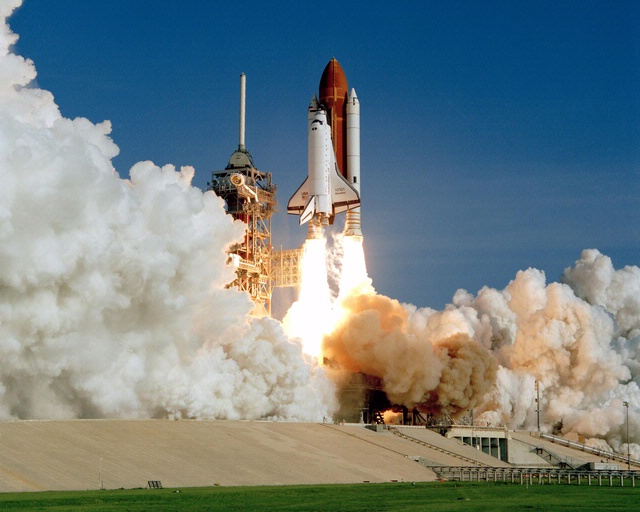
\includegraphics[scale=0.35]{gambar/roketluarangkasa.jpg}

  % Ubah dengan keterangan gambar yang diinginkan
  \caption{Peluncuran roket luar angkasa \emph{Discovery} \parencite{roketluarangkasa}.}
  \label{fig:roketluarangkasa}
\end{figure}

Roket luar angkasa merupakan \lipsum[1]

\emph{Discovery}, Gambar \ref{fig:roketluarangkasa}, merupakan \lipsum[2]

\section{Gravitasi}
\label{sec:gravitasi}

Gravitasi merupakan \lipsum[1]

\subsection{Hukum Newton}
\label{subsec:hukumnewton}

Newton \parencite{newton1687} pernah merumuskan bahwa \lipsum[1]
Kemudian menjadi persamaan seperti pada persamaan \ref{eq:hukumpertamanewton}.

% Contoh pembuatan persamaan
\begin{equation}
  \label{eq:hukumpertamanewton}
  \sum \mathbf{F} = 0\; \Leftrightarrow\; \frac{\mathrm{d} \mathbf{v} }{\mathrm{d}t} = 0.
\end{equation}

\subsection{Anti Gravitasi}
\label{subsec:antigravitasi}

Anti gravitasi merupakan \lipsum[1]

\cleardoublepage

% Bab 3 desain dan implementasi
\chapter{DESAIN DAN IMPLEMENTASI}
\label{chap:desainimplementasi}

% Ubah bagian-bagian berikut dengan isi dari desain dan implementasi

Penelitian ini dilaksanakan sesuai \lipsum[1][1-5]

\section{Deskripsi Sistem}
\label{sec:deskripsisistem}

Sistem akan dibuat dengan \lipsum[1-2]

\section{Implementasi Alat
  \label{sec:implementasi alat}}

Alat diimplementasikan dengan \lipsum[1]

% Contoh pembuatan potongan kode
\begin{lstlisting}[
  language=C++,
  caption={Program halo dunia.},
  label={lst:halodunia}
]
#include <iostream>

int main() {
    std::cout << "Halo Dunia!";
    return 0;
}
\end{lstlisting}

\lipsum[2-3]

% Contoh input potongan kode dari file
\lstinputlisting[
  language=Python,
  caption={Program perhitungan bilangan prima.},
  label={lst:bilanganprima}
]{program/bilangan-prima.py}

\lipsum[4]

\cleardoublepage

% Bab 4 pengujian dan analisis
\chapter{HASIL DAN PEMBAHASAN}

% Ubah bagian-bagian berikut dengan isi dari pengujian dan analisis

Pada bab ini dipaparkan hasil dan analisa dari pelaksanaan tiap tahap pada metodologi, skenario pengujian dan evaluasi pengujiannya. Pengujian dan evaluasi dilakukan guna mengetahui tingkat kesalahan dalam metodologi serta ananlisis untuk mencapai kesimpulan.Tahapan scenario pengujian meliputi hal berikut :

\begin{enumerate}
  \item Pengujian akurasi model dalam beberapa situasi
  \item Pengujian interaksi model pada beberapa responden
  \item Pengujian pada robot dengan beberapa kondisi
\end{enumerate}
Dengan hasil metodologi serta pelaksanaan skenario-skenario pengujian yang dipaparkan pada bab Penelitian dan pembahasan, diharapkan mendapatkan hasil dan analisa sehingga dapatditarik kesimpulan dari pelaksanaan tugas akhir ini.

\section{Hasil metodologi}
Pada metodologi terdapat blok diagaram sebagai acuan dalam Penelitian yang telah dilaksanakan. Adapun hasil dari blok diagram tersebut secara rinci sebagai berikut :

\subsection{Hasil dataset}
Proses pengumpulan dataset dilakukan dengan pengambilan citra menggunakan kamera. Proses tersebut dilakukan selama beberapa waktu untuk dapat mendapatkan beberapa frame citra untuk suatu class dan diulang kembali dengan class yang berbeda sampai seluruh class terpenuhi. Seluruh citra tangan diambil dari satu orang yang sama dan menggunakan jarak pengambilan yang sama, yaitu jarak antara kamera dan tangan. Dalam proses pengambilan citra dilakukan beberapa variasi dalam pose tangan yaitu dengan sedikit merotasikan tangan dan sedikit melemaskan tangan. Hal ini dilakukan agar tiap class memiliki variasi pose dan dapat mendeteksi dari berbagai kondisi pose. Adapun pose yang digunakan sebagai dataset dapat dilihat pada Tabel \ref{tab:citradaset}.

\begin{table}[H]
  \centering
  \caption{Citra hasil dataset}
  \label{tab:citradaset}
  \begin{tabular}{|c|c|}
  \hline
  Pose   & Citra \\ \hline
  Diam   & 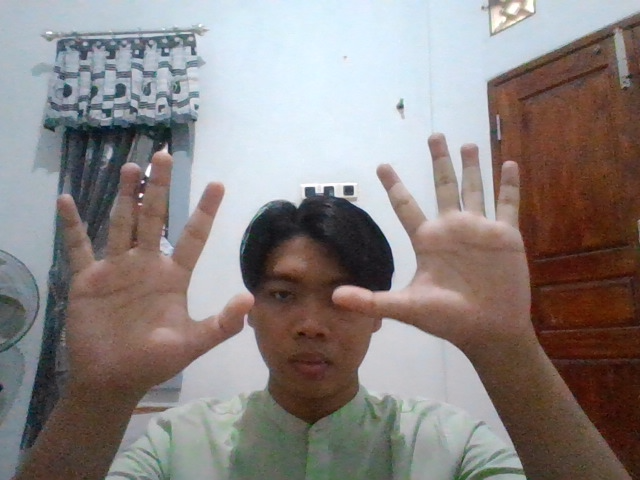
\includegraphics[width=0.3\linewidth]{gambar/posediam.png} \\ \hline
  Kanan  & 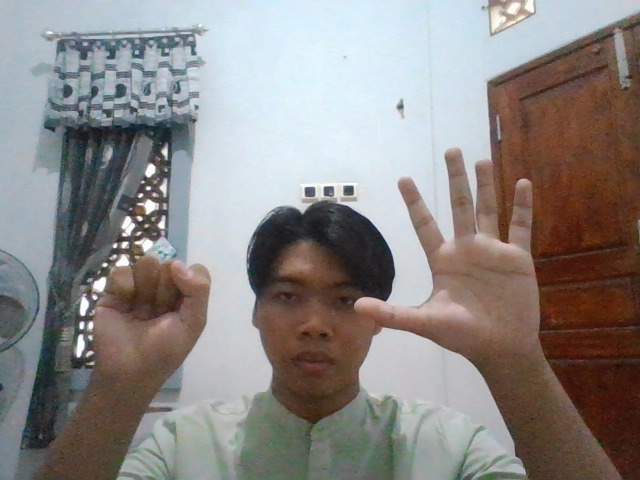
\includegraphics[width=0.3\linewidth]{gambar/posekanan.png} \\ \hline
  Kiri   & 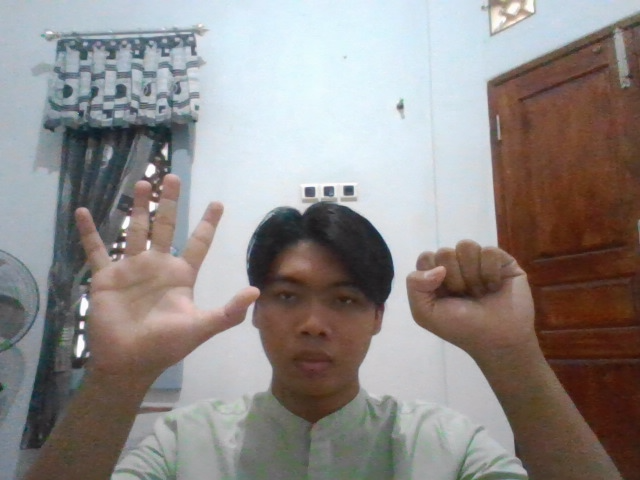
\includegraphics[width=0.3\linewidth]{gambar/posekiri.png} \\ \hline
  Maju   & 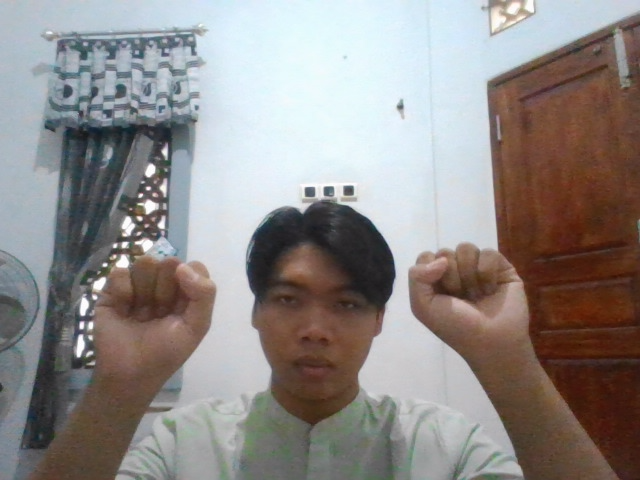
\includegraphics[width=0.3\linewidth]{gambar/posemaju.png} \\ \hline
  Mundur & 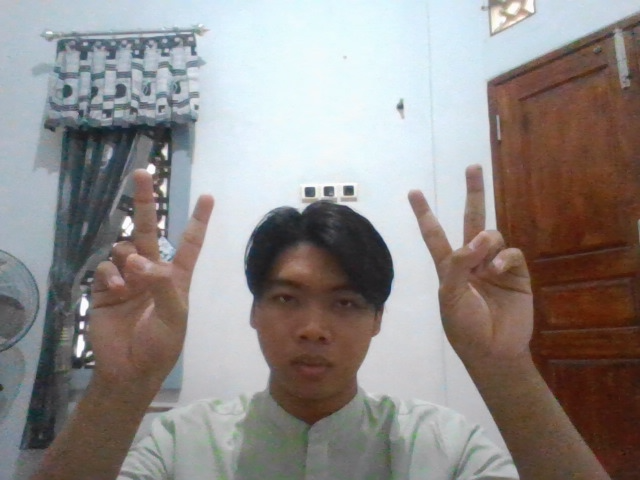
\includegraphics[width=0.3\linewidth]{gambar/posemundur.png} \\ \hline
  Tembak & 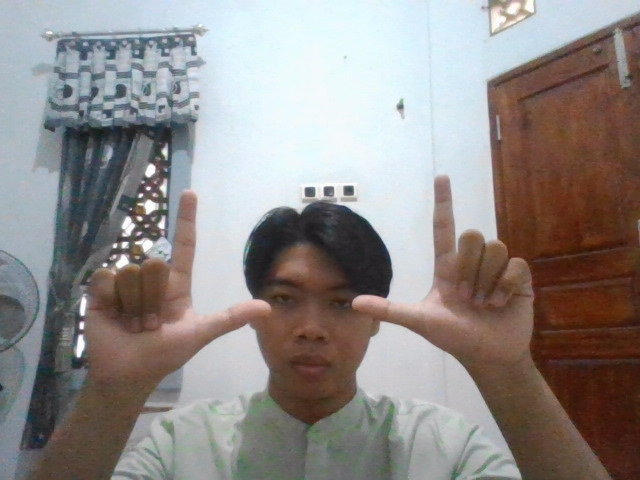
\includegraphics[width=0.3\linewidth]{gambar/posetembak.png} \\ \hline
\end{tabular}
\end{table}


\subsection{Hasil Pose \emph{Prediction}}

\begin{figure}[H]
  \centering
  \begin{tabular}{cc}
    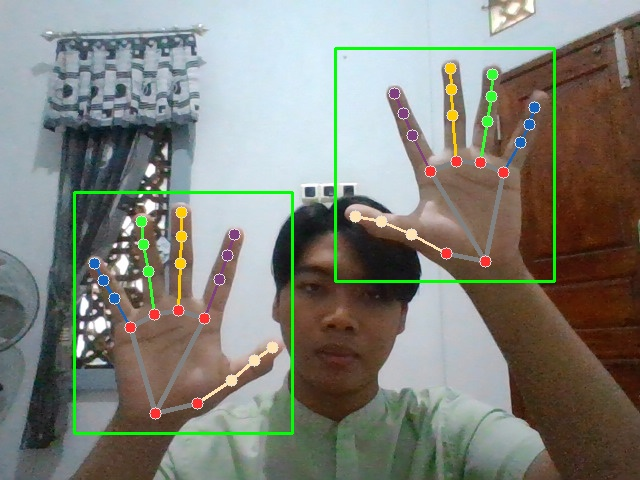
\includegraphics[width=0.4\linewidth]{gambar/hasilposepred.jpg} & 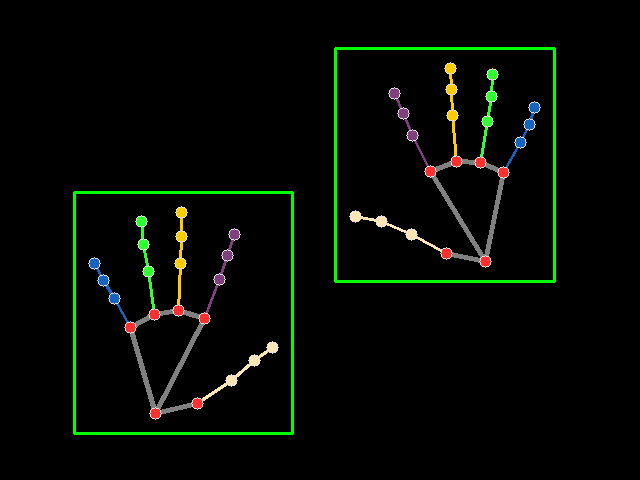
\includegraphics[width=0.4\linewidth]{gambar/hasilposepredhitam.png} \\
    a. Citra berwarna & b. Citra hitam 
    \end{tabular}
    \caption{Hasil\emph{ hand landmark}}
  \label{fig:hasilposepred}
\end{figure}

Proses pose \emph{prediction} dilakukan dengan menggambar \emph{hand landmark} yang telah terdeteksi dengan menggunakan \emph{Mediapipe} pada tiap-tiap citra yang telah dikumpulan pada tahap sebelumnya. Setelah \emph{hand landmark} tergambar maka tiap-tiap \emph{hand landmark} digambar pada citra berlatar gelap. Hasil dari \emph{hand landmark} pada citra hasil kamera dan citra hitam dapat dilihat pada Gambar \ref{fig:hasilposepred}. \emph{Hand landmark} yang terdapat pada citra ini diberikan \emph{bounding box} pada tiap tangan. Setelah \emph{bounding box} terbuat maka selanjutnya dilakukan \emph{hand localization} pada \emph{hand landmark} yang berada pada citra hitam. \emph{Hand} \emph{localization} ini untuk mengecilkan ukuran citra menjadi hanya selebar \emph{bounding box} dengan ditambah 20 \emph{pixel} pada nilai maksimal dan dikurangi 20 \emph{pixel} pada nilai minimum pada tiap \emph{bounding box}. Penambahan \emph{pixel} ini dimaksudkan untuk mencakup semua \emph{hand landmark} yang telah dibuat \emph{Mediapipe}. Dengan mengurangi ukuran citra ini bertujuan mengurangi waktu training dan dapat meningkatkan performa. Citra diluar \emph{bounding box} dibuang dan tiap \emph{bounding box} dirubah ukurannya menjadi 128x128 \emph{pixel} untuk menyamakan kedua \emph{bounding box} dalam satu frame citra. Setelah setiap ukuran \emph{bounding box} sama maka setiap \emph{bounding box} ditumpuk secara horizontal. Citra yang disimpan dan dijadikan dataset adalah citra yang terdapat dua \emph{hand landmark} yang telah ditumpuk secara horizontal. Citra yang disimpan nantinya memiliki ukuran 256x128 \emph{pixel} dikarenakan hasil dari dua tangan yang terdeteksi. Pada tahap menumpuk citra terdapat dua macam tumpukan yaitu citra dengan posisi tangan kiri berada pada kotak sebelah kiri dan tangan kanan pada kotak sebelah kanan. Posisi kedua yaitu tangan kiri berada pada posisi kanan dan tangan kanan berada pada kiri yang selanjutnya disebut sebagai posisi invers. Posisi \emph{hand landmark} dari hasil hand localization dapat dilihat pada Tabel \ref{tab:posisigtangan}.

\begin{table}[H]
  \centering
  \caption{Hasil posisi hand localization}
  \label{tab:posisigtangan}
  \begin{tabular}{|c|c|c|}
  \hline
  Pose   &Pose Benar&Pose Invers\\ \hline
  Diam   & 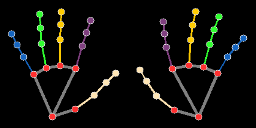
\includegraphics[width=0.3\linewidth]{gambar/Diam (1).png} & 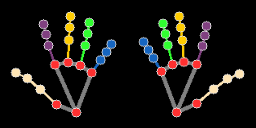
\includegraphics[width=0.3\linewidth]{gambar/DiamI (1).png} \\ \hline
  Kanan  & 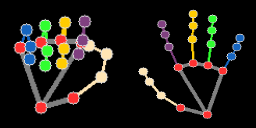
\includegraphics[width=0.3\linewidth]{gambar/Kanan (1).png} & 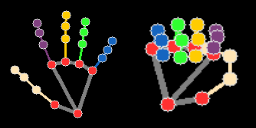
\includegraphics[width=0.3\linewidth]{gambar/KananI (1).png} \\ \hline
  Kiri   & 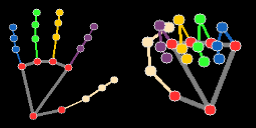
\includegraphics[width=0.3\linewidth]{gambar/Kiri (1).png} & 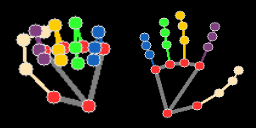
\includegraphics[width=0.3\linewidth]{gambar/KiriI (1).png} \\ \hline
  Maju   & 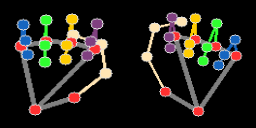
\includegraphics[width=0.3\linewidth]{gambar/Maju (1).png} & 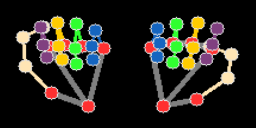
\includegraphics[width=0.3\linewidth]{gambar/MajuI (1).png} \\ \hline
  Mundur & 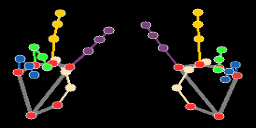
\includegraphics[width=0.3\linewidth]{gambar/Mundur (1).png} & 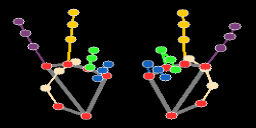
\includegraphics[width=0.3\linewidth]{gambar/MundurI (1).png} \\ \hline
  Tembak & 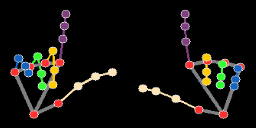
\includegraphics[width=0.3\linewidth]{gambar/Tembak (1).png} & 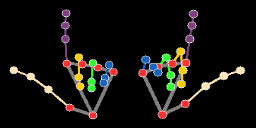
\includegraphics[width=0.3\linewidth]{gambar/TembakI (1).png} \\ \hline
  \end{tabular}
\end{table}




\subsection{Hasil \emph{Classification}}
Proses classification dimulai dari \emph{training} dataset. Sebelum melakukan \emph{training} maka dibutuhkannya data citra pada tiap class. Tiap class memiliki \emph{train data} dan \emph{validation data}. Data-data ini diambil dari proses sebelumnya yaitu citra yang telah melewati tahap hand localization. Citra untuk train data pada tiap class berjumlah 400 dengan rincian 200 citra posisi benar dan 200 citra posisi invers, sedangkan citra untuk \emph{validation data} berjumlah 80 citra dengan 40 citra posisi benar dan 40 citra posisi invers. Adapaun tabel pesebaran data citra tiap class dapat dilihat pada Tabel \ref{tab:tiapclass}. \emph{Training} ini menggunakan CNN dengan menggunakan satu layer \emph{convolution} ukuran 3x3 dengan filter 16, sehingga ukuran citra yang awalnya 256x128 turun menjadi 254x126 yang disebabkan dari adanya konvolusi. Selanjutnya dilakukan \emph{pooling} dengan menggunakan \emph{max} \emph{pooling} ukuran 2x2 yang menyebabkan ukuran citra turun menjadi setengah dari hasil konvolusi yaitu 167x63. Layer selanjutnya yaitu \emph{flatten} dimana citra hasil dari max pooling di ubah menjadi vektor. Output yang didapatkan dari layer \emph{flatten} yaitu 128016 vektor.  Setelah di tentukannya konfigurasi layer CNN maka tahapan selanjutnya yaitu konfigurasi hyperparameter. Adapun konfigurasi pada hyperparameter yang digunakan dapat dilihat pada Tabel \ref{fig:hyperparameter} berikut.

\begin{table}[H]
  \centering
  \caption{Jumlah Citra Tiap \emph{Class}}
  \label{tab:tiapclass}
  \begin{tabular}{|c|c|c|}
  \hline
  \emph{Class}  & Train Data & Validation Data \\ \hline
  Diam   & 400        & 80              \\ \hline
  Kanan  & 400        & 80              \\ \hline
  Kiri   & 400        & 80              \\ \hline
  Maju   & 400        & 80              \\ \hline
  Mundur & 400        & 80              \\ \hline
  Tembak & 400        & 80              \\ \hline
  \end{tabular}
\end{table}

\begin{table}[H]
  \centering
  \caption{Konfigurasi \emph{hyperparameter}}
  \label{fig:hyperparameter}
  \begin{tabular}{|c|c|lll}
  \cline{1-2}
  \emph{Hyperparameter} & Konfigurasi \\ \cline{1-2}
  Epochs         & 20 \\ \cline{1-2}
  Batchsize      & 32 \\ \cline{1-2}
  Image Size     & 256x128 \\ \cline{1-2}
  Step per epoch      & 75 \\ \cline{1-2}
  Optimizer      & Adam \\ \cline{1-2}
  \end{tabular}
\end{table}

Setelah proses konfigurasi layer CNN dan \emph{hyperparameter} telah dilakukan. Selanjutnya yaitu proses \emph{training} yaitu berupa model dan detail data pada tiap proses pengulangan. Hasil dari \emph{training} ini didapatkan \emph{training} \emph{accuracy}, \emph{validation} \emph{accuracy}, \emph{training} \emph{loss}, dan \emph{validation} \emph{loss}. Setiap perulangan mendapatkan nilai tersebut, grafik dari nilai tersebut dalam 20 perulangan dapat dilihat pada Gambar \ref*{fig:loss} dan Gambar \ref*{fig:akurasi}

\begin{figure}[H]
  \centering
  \includegraphics[width=0.7\linewidth]{gambar/loss.png}
  \caption{Grafik \emph{training} dan \emph{validation} \emph{loss}}
  \label{fig:loss}
\end{figure}

\begin{figure}[H]
  \centering
  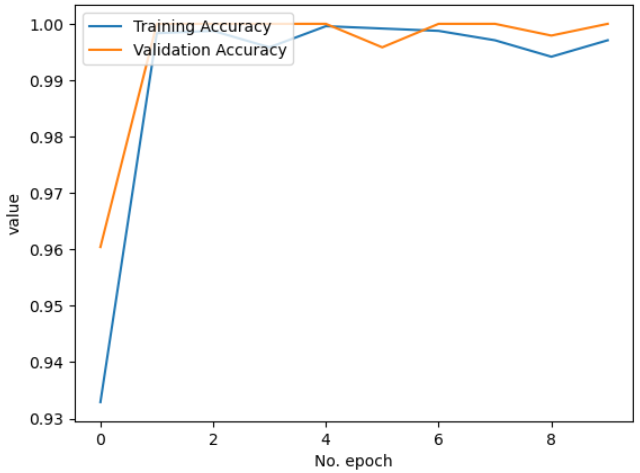
\includegraphics[width=0.7\linewidth]{gambar/akurasi.png}
  \caption{Grafik \emph{training} dan \emph{validation} \emph{accuracy}}
  \label{fig:akurasi}
\end{figure}

Setelah proses \emph{training} selesai dan telah didapatkan model dengan akurasi yang tinggi atau sesuai \emph{threshold} dalam hal ini dapat dilihat pada grafik akurasi pada Gambar \ref{fig:akurasi}, maka selanjutnya masuk kepada proses evaluasi model. Evaluasi model menggunakan \emph{confusion matrix} dengan data testing citra sebanyak 100 pada masing-masing class. Hasil dari \emph{confusion matrix} didapatkan akurasi 0.95. Hasil evaluasi dengan \emph{confusion matrix} secara lengkap dapat dilihat pada Gambar \ref{fig:confusionmatrix}. Model yang telah dievaluasi menggunakan \emph{confusion matrix} selanjutnya digunakan sebagai \emph{classification}. \emph{Classification} menghasilkan kode instruksi yang digunakan sebagai acuan dalam memberikan perintah kepada robot. Adapun kode instruksi yang diatur sebagai perintah kepada robot dapat dilihat pada Tabel \ref{tab:kodeinstruksi}

\begin{figure}[H]
  \centering
  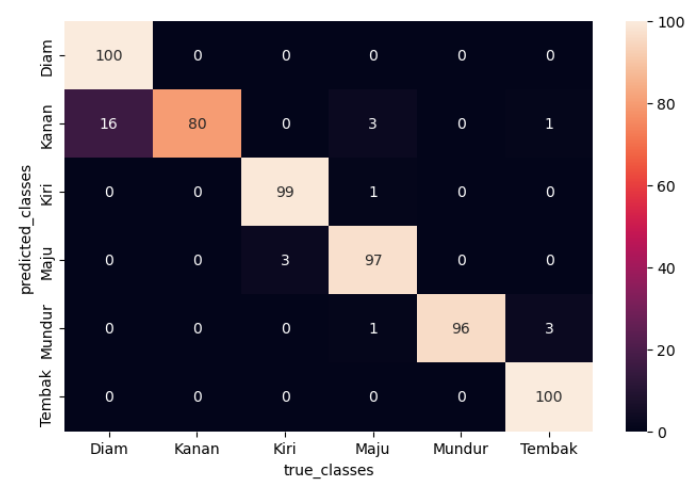
\includegraphics[width=0.7\linewidth]{gambar/confusionmatrix.png}
  \caption{Hasil \emph{Confusion Matrix}}
  \label{fig:confusionmatrix}
\end{figure}

\begin{table}[H]
  \centering
  \caption{Kode instruksi hasil \emph{classification}}
  \label{tab:kodeinstruksi}
  \begin{tabular}{|c|c|}
  \hline
  Pose   & Kode Instruksi \\ \hline
  Diam   & n              \\ \hline
  Kanan  & r              \\ \hline
  Kiri   & l              \\ \hline
  Maju   & f              \\ \hline
  Mundur & b              \\ \hline
  Tembak & s              \\ \hline
  \end{tabular}
\end{table}

\subsection{\emph{Control Navigation}}
Proses \emph{control navigation} diawali dengan perancangan pada robot. Robot dirancang dengan memiliki kemampuan untuk bergerak dan menembak. Pergerakan robot dapat terjadi dikarenakan adanya sepasang roda yang dipasangkan pada robot. Perputaran roda diatur dari motor driver dengan menyalurkan listrik kepada motor dc yang sudah dipasangkan roda sebagai outputya. Kemampuan menembak pada robot diatur dengan adanya sensor \emph{infrared}. Sensor \emph{infrared transmitter} diletakkan didepan robot sedangakn sensor \emph{infrared receiver} membutuhkan empat yang diletakkan disekeliling sisi robot. Sensor infrared receiver akan di sambungkan secara pararel untuk ke empat sensornya dan dihubungkan kepada mikrokontroler dalam hal ini yang digunakan adalah "nodeMCU ESP8266". Secara schematic dapat dilihat pada Gambar \ref{fig:schematic}. Robot yang telah dirancang selanjutnya diuji dengan cara mengirimkan kode instruksiyang dihasilkan dari proses \emph{classification} kepada mikrokontroler robot. Pengujian ini dilakukan dengan mengklasifikasi 20 citra pada tiap class. Pengujian ini bertujuan untuk mengetahuiapakah ada data yang tidak terkirim atau hilang saat dikirim. Hasil dari klasifikasi akan dirubah menjadi kode instruksi dan dikirim kepada mikrokontroler. Pada mikrokontroler dihitung jumlah kode instruksi yang masuk dan dibandingkan dengan kode yang dikirim. Hasil pengujian ini dapat dilihat pada Tabel \ref{tab:hasulujipose}

\begin{table}[H]
  \centering
  \caption{Hasil uji komunikasi laptop dengan robot}
  \label{tab:hasulujipose}
  \begin{tabular}{|c|c|}
  \hline
  Pose   &  Hasil Uji\\ \hline
  Diam   & 20              \\ \hline
  Kanan  & 20             \\ \hline
  Kiri   & 20              \\ \hline
  Maju   & 20              \\ \hline
  Mundur & 20              \\ \hline
  Tembak & 20              \\ \hline
  \end{tabular}
\end{table}

\begin{figure}[H]
  \centering
  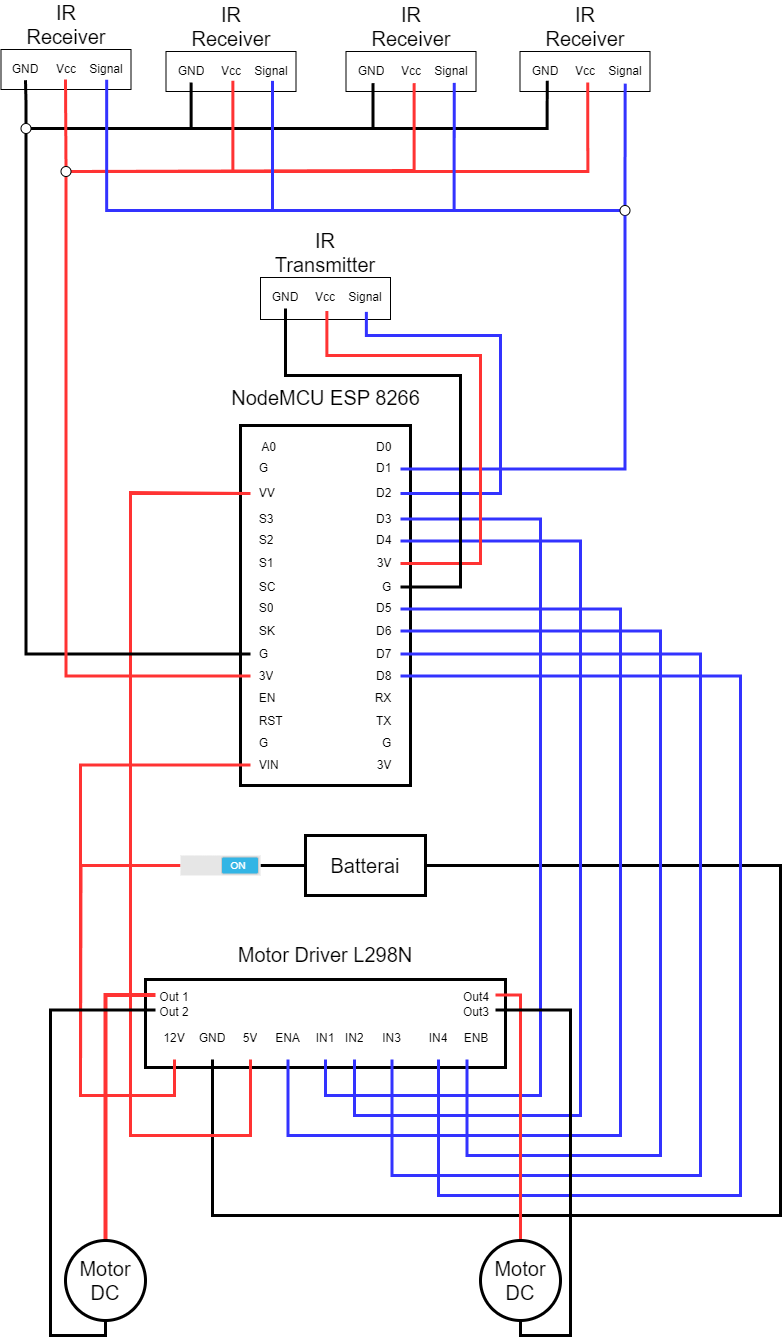
\includegraphics[width=0.5\linewidth]{gambar/schematic.png}
  \caption{\emph{Schematic} robot}
  \label{fig:schematic}
\end{figure}

\section{Skenario pengujian}
Pada skenario pengujian dilakukan beberapa skenario pengujian untuk mengetahui tingkat kesalahan dan membuka potensi pengembangan penelitian serta menarik kesimpulan secara keseluruhan. Skenario pegujian yang dilakukan yaitu sebagai berikut :
\subsection{Pengujian akurasi model}
Pengujian akurasi model bertujuan untuk membandingkan akurasi model dalam beberapa situasi uji guna mengetahui situasi ideal untuk melakukan classification. Pengujian ini menggunakan tangan peneliti dengan variasi jarak tangan terhadap kamera, intensitas cahaya ruangan, dan sudut kamera terhadap tangan. Hasil dari pengujian tersebut secara spesifik sebagai berikut :
\begin{enumerate}
  \item Pengujian jarak \\
  Pengujian jarak dilakukan dengan cara mengambil 20 citra dari tiap \emph{class} pada jarak tertentu. Jarak ini dimulai dari 30cm, 50cm, dan 100cm antara tangan dengan kamera. Pengujian dilakukan karena adanya perubahan bentuk dari \emph{hand landmark}. Hasil pose yang terdeteksi dari pengujian jarak dapat dilihat pada Tabel \ref{tab:hasiljarak}

  \begin{table}[H]
    \centering
    \caption{Pose yang terdeteksi dari pengujian jarak}
    \label{tab:hasiljarak}
    \begin{tabular}{|c|clll|}
      \hline
      \multirow{2}{*}{Pose} & \multicolumn{4}{c|}{Jarak (cm)}                                                   \\ \cline{2-5} 
                            & \multicolumn{1}{l|}{30} & \multicolumn{1}{l|}{50} & \multicolumn{1}{l|}{80} & 100 \\ \hline
      Diam                  & \multicolumn{1}{c|}{20}   & \multicolumn{1}{l|}{19}   & \multicolumn{1}{l|}{20}   &   20  \\ \hline
      Kanan                 & \multicolumn{1}{c|}{20}   & \multicolumn{1}{l|}{20}   & \multicolumn{1}{l|}{16}   &   10  \\ \hline
      Kiri                  & \multicolumn{1}{c|}{19}   & \multicolumn{1}{l|}{20}   & \multicolumn{1}{l|}{20}   &   20  \\ \hline
      Maju                  & \multicolumn{1}{c|}{19}   & \multicolumn{1}{l|}{20}   & \multicolumn{1}{l|}{20}   &   20  \\ \hline
      Mundur                & \multicolumn{1}{c|}{20}   & \multicolumn{1}{l|}{20}   & \multicolumn{1}{l|}{20}   &   20  \\ \hline
      Tembak                & \multicolumn{1}{c|}{20}   & \multicolumn{1}{l|}{20}   & \multicolumn{1}{l|}{15}   &   10  \\ \hline
      Akurasi                  & \multicolumn{1}{c|}{0.95}   & \multicolumn{1}{l|}{0.99}   & \multicolumn{1}{l|}{0.93}   &   0.83  \\ \hline
    \end{tabular}
  \end{table}

  \begin{figure}[H]
      \begin{tabular}{cccc}
        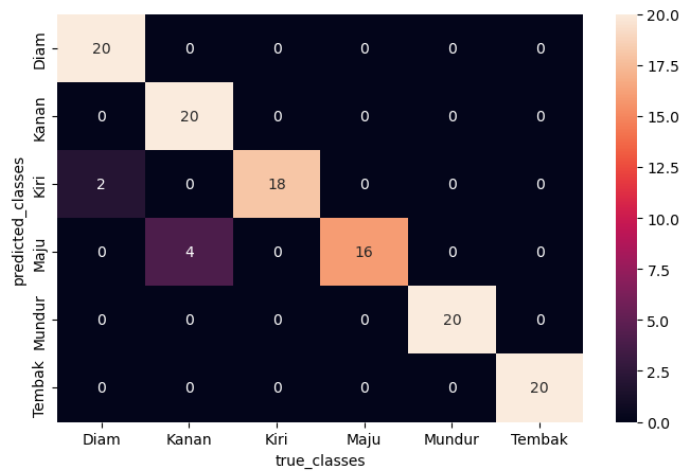
\includegraphics[width=0.4\linewidth]{gambar/cm30.png} & 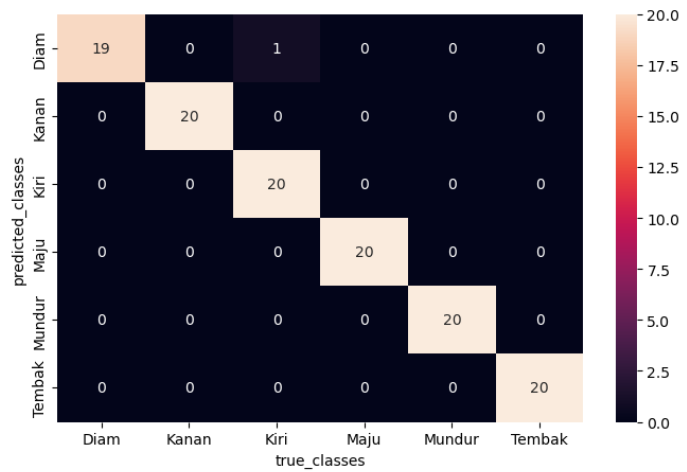
\includegraphics[width=0.4\linewidth]{gambar/cm50.png} \\
        a. Jarak 30cm & b. Jarak 50cm \\ 
        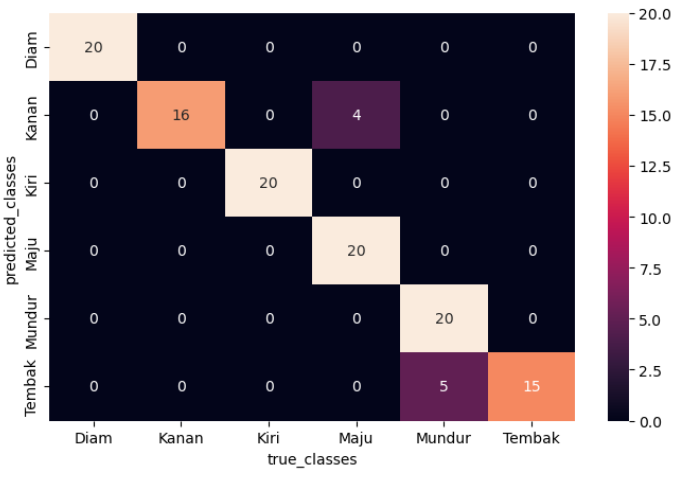
\includegraphics[width=0.4\linewidth]{gambar/cm80.png} & 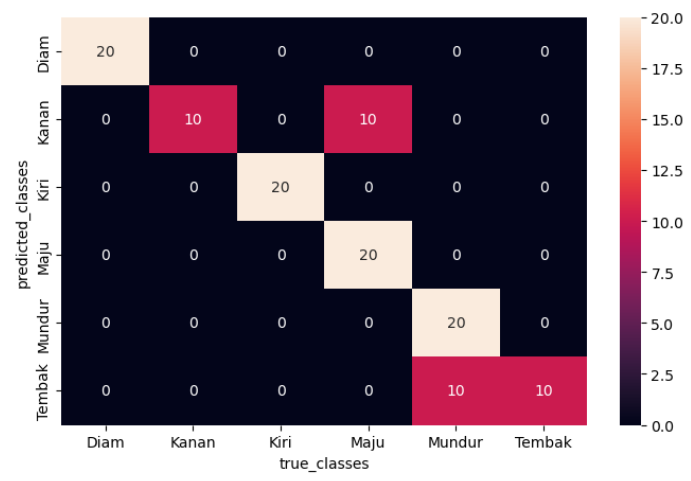
\includegraphics[width=0.4\linewidth]{gambar/cm100.png} \\
        c. Jarak 80cm & d. Jarak 100cm
      \end{tabular}
      \centering
      \caption{Pengujian \emph{Confussion Matrix} pada jarak tertentu}
      \label{fig:confusionmatrixjarak}
  \end{figure}
  

  % \item Pengujian intensitas cahaya \\
  % Pengujian intensitas cahaya 
  % \item Pengujian sudut kamera \\
\end{enumerate}
\cleardoublepage

% Bab 5 penutup
% \chapter{PENUTUP}
\label{chap:penutup}

% Ubah bagian-bagian berikut dengan isi dari penutup
Pada bab ini akan dipaparkan kesimpulan dari hasil pengujian yang akan menjawab dari permasalahan yang diangkat oleh pelaksanaan tugas akhir ini. Pada bab ini juga dipaparkan saran mengenai hal yang dapat dilakukan untuk mengembangkan penelitian kedepannya.

\section{Kesimpulan}
\label{sec:kesimpulan}

 Berdasarkan hasil penelitian yang telah dipaparkan pada Bab 4 dapat disimpulak bahwa :

\begin{enumerate}[nolistsep]

  \item Arsitektur CNN dapat digunakan untuk klasifikasi tangan hasil  \emph{hand landmark} menggunakan \emph{Mediapipe} didapatkan nilai akura sebesar 0.95

  \item Pengujian akurasi menggunakan variasi jarak didapatkan hasil bahwa jarak ideal didapatkan pada jarak 50cm antara tangan dengan kamera.


\end{enumerate}

\section{Saran}
\label{chap:saran}

Untuk pengembangan lebih lanjut pada \lipsum[1][1-3] antara lain:

\begin{enumerate}[nolistsep]

  \item Memperbaiki \lipsum[2][1-3]

  \item \lipsum[2][4-6]

  \item \lipsum[2][7-10]

\end{enumerate}

% \cleardoublepage

\chapter*{DAFTAR PUSTAKA}
\addcontentsline{toc}{chapter}{DAFTAR PUSTAKA}
\renewcommand\refname{}
\vspace{2ex}
\renewcommand{\bibname}{}
\begingroup
\def\chapter*#1{}
\printbibliography
\endgroup
\cleardoublepage

% Biografi penulis
\begin{center}
  \Large
  \textbf{BIOGRAFI PENULIS}
\end{center}

\addcontentsline{toc}{chapter}{BIOGRAFI PENULIS}

\vspace{2ex}

\begin{wrapfigure}{L}{0.3\textwidth}
  \centering
  \vspace{-3ex}
  % Ubah file gambar berikut dengan file foto dari mahasiswa
  
\includegraphics[width=0.3\textwidth]{gambar/elon.jpg}
  \vspace{-4ex}
\end{wrapfigure}

% Ubah kalimat berikut dengan biografi dari mahasiswa
\name{}, lahir pada \lipsum[1]

\lipsum[2]

\cleardoublepage

\end{document}